%\documentclass[aspectratio=34]{beamer}
\documentclass{beamer}

% Remove the gratuituous footer
\setbeamertemplate{footline}{}
\setbeamertemplate{navigation symbols}{}
%\renewcommand{\insertnavigation}[1]{}

\usepackage{rotating}
\usepackage{subfigure}
\usepackage{algorithm}
\usepackage{algorithmicx}
\usepackage{algpseudocode}
\usepackage{xcolor}

\usepackage{graphicx}
\DeclareMathOperator{\conv}{conv}
\DeclareMathOperator{\st}{s.t.}
\DeclareMathOperator{\dom}{dom}
\DeclareMathOperator{\im}{im}
\DeclareMathOperator{\Ne}{Ne}
\DeclareMathOperator{\sign}{sign}
\DeclareMathOperator{\Var}{Var}
\DeclareMathOperator{\diag}{diag}
\DeclareMathOperator{\vvec}{vec}


%\usepackage{beamerthemesplit}

% Make footnotes visible. Stolen from http://tex.stackexchange.com/questions/5852/beamer-footnote-text-collides-with-navigation-symbols
\addtobeamertemplate{footnote}{\vspace{-6pt}\advance\hsize-0.5cm}{\vspace{6pt}}
\makeatletter
% Alternative A: footnote rule
\renewcommand*{\footnoterule}{\kern -3pt \hrule \@width 2in \kern 8.6pt}
% Alternative B: no footnote rule
% \renewcommand*{\footnoterule}{\kern 6pt}
\makeatother

\setbeamertemplate{bibliography item}{}
\usepackage[style=authoryear-comp,natbib=true,firstinits,doi=true,isbn=false,url=false,eprint=false,backend=biber]{biblatex}
%\usepackage[sorting=none,firstinits,doi=false,isbn=false,url=false,backend=biber]{biblatex}
\bibliography{ML}
% Don't display series
\AtEveryBibitem{\clearlist{series}}
\AtEveryBibitem{\clearfield{series}}
\DeclareSourcemap{
  \maps[datatype=bibtex]{
    \map{
       \step[fieldset=series, null]
    }
  }
}

\DeclareFieldFormat{titlecase}{\MakeTitleCase{#1}}

% Correct casing for journal titles.
\newrobustcmd{\MakeTitleCase}[1]{%
  \ifthenelse{\ifcurrentfield{booktitle}\OR\ifcurrentfield{booksubtitle}%
    \OR\ifcurrentfield{maintitle}\OR\ifcurrentfield{mainsubtitle}%
    \OR\ifcurrentfield{journaltitle}\OR\ifcurrentfield{journalsubtitle}%
    \OR\ifcurrentfield{issuetitle}\OR\ifcurrentfield{issuesubtitle}%
    \OR\ifentrytype{book}\OR\ifentrytype{mvbook}\OR\ifentrytype{bookinbook}%
    \OR\ifentrytype{booklet}\OR\ifentrytype{suppbook}%
    \OR\ifentrytype{collection}\OR\ifentrytype{mvcollection}%
    \OR\ifentrytype{suppcollection}\OR\ifentrytype{manual}%
    \OR\ifentrytype{periodical}\OR\ifentrytype{suppperiodical}%
    \OR\ifentrytype{proceedings}\OR\ifentrytype{mvproceedings}%
    \OR\ifentrytype{reference}\OR\ifentrytype{mvreference}%
    \OR\ifentrytype{report}\OR\ifentrytype{thesis}}
    {#1}
{\MakeSentenceCase{#1}}}

%%%%%%%%%%%%%%%%%%%%%%%%%%%%%%%%%%%%%%%%%%%%%%%%%%%%%%%%%%%%%%%%%%%%
%% THE ACTUAL DOCUMENT BEGINS
%%%%%%%%%%%%%%%%%%%%%%%%%%%%%%%%%%%%%%%%%%%%%%%%%%%%%%%%%%%%%%%%%%%%

\title{Topic Models for Texts and Images in Representation Space}
\author{Kui Tang and Sameer Lal}
\institute{Columbia University}

\date{15 April 2015}

\begin{document}

\frame{\titlepage}

\begin{frame}
  \frametitle{Topic Models}
  {\centering 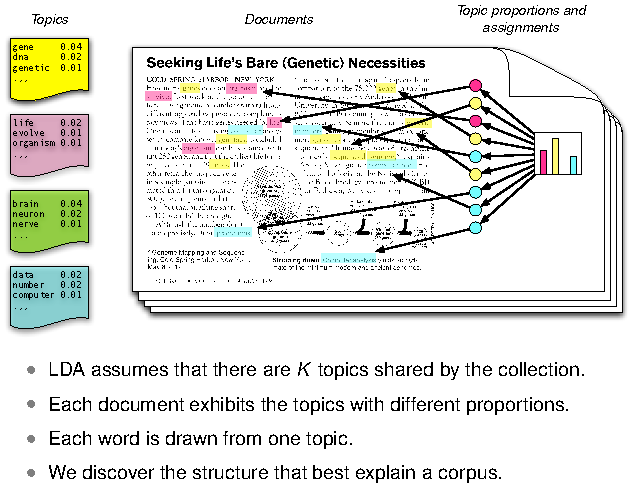
\includegraphics[width=\textwidth]{assets/lda_colors.pdf}}
  {\small \emph{Slide stolen from D. Blei.} \par}
\end{frame}

\begin{frame}
  \frametitle{Latent Variable Models}
  {\centering 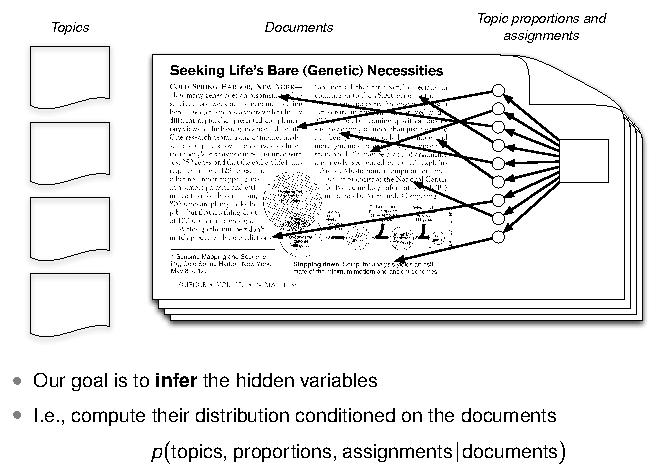
\includegraphics[width=\textwidth]{assets/lda_hidden.pdf}}
  {\small \emph{Slide stolen from D. Blei.} \par}
\end{frame}

\begin{frame}
  \frametitle{Bayesian Networks}
  {\centering 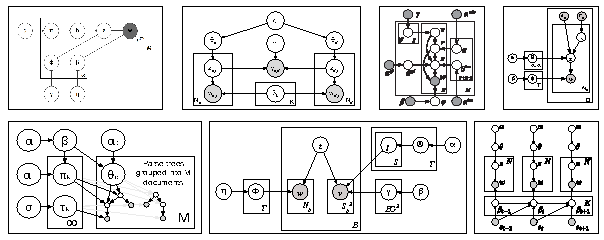
\includegraphics[width=\textwidth]{assets/lda_crazy.pdf}}
  {\small \emph{Slide stolen from D. Blei.} \par}
  \begin{itemize}
  \item Shaded variables are \emph{observed}, other variables are \emph{hidden}.
  \item A model is our hypothesis for how data are generated.
  \item We \emph{condition} on observations to update our hypothesis.
  \end{itemize}
\end{frame}


\begin{frame}
  \frametitle{Multimodal Documents}
  \begin{center}
    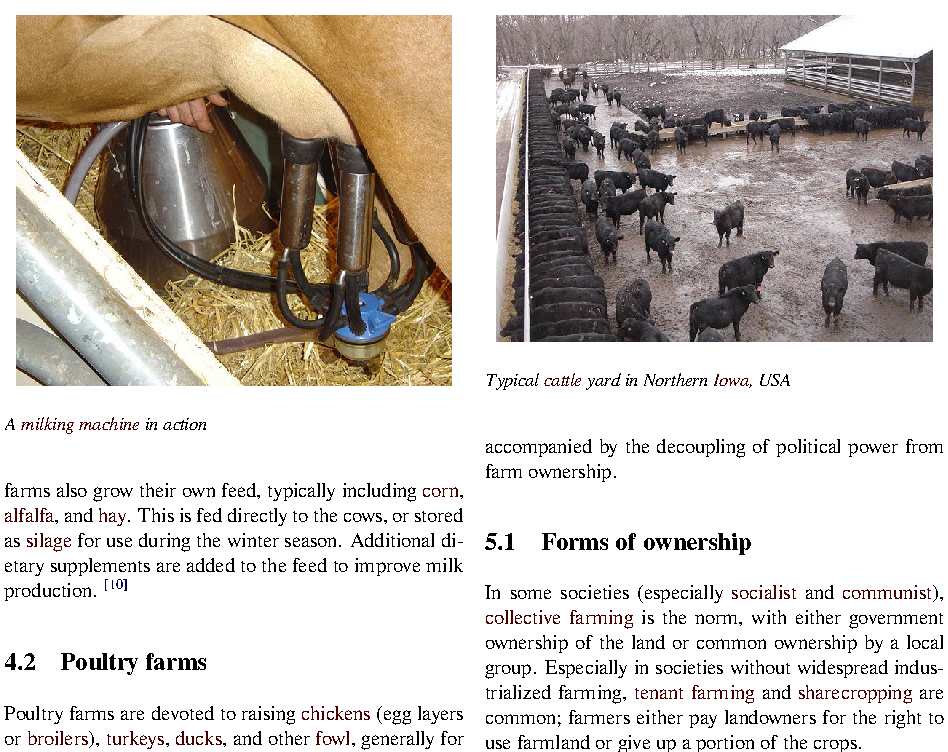
\includegraphics[width=0.75\textwidth]{assets/wiki_farm.pdf}
  \end{center}
             
  \begin{itemize}
  \item \emph{We want to learn a topic model using text and images jointly.}
  \item Images and text complement each other.
  \item Captions aren't the whole story: cows in political contexts.
  \end{itemize}
             
\end{frame}

\begin{frame}
  \frametitle{Gaussian Topic Models with CNNs}
  \begin{center}
    \includegraphics[width=0.7\textwidth]{gtm_cnn.pdf}
  \end{center}
  {\small
  \begin{itemize}
  \item Topics are (mixtures of) Gaussians.
  \item Words are latent vectors $\lambda_v \in \mathbb{R}^{D_W}$ using Bayesian word2vec.
  \item Images are latent vectors $v_{in} \in \mathbb{R}^{D_I}$ \emph{conditioned} on raw images $x_{di}$. We have $v_{ni} \sim \mathcal{N}(M \text{CNN}_x(x_{ni} ; \Omega), \Sigma)$ with $\Omega$ CNN parameters, $M$ mapping to word vector space, and $\text{CNN}_x$ feature representation output by CNN.
  \end{itemize}
  \par}
\end{frame}

\begin{frame}
  \frametitle{Aligning Image and Word Vectors}
  \begin{itemize}
    \item Image vectors $v_{ni}$ are 4096 dimensional CNN representation layer, prior to fully connected classification layers.
    \item Represent high-level semantic information about image.
    \item Word vectors $w_{dn}$ are {100, 300, 500, 1000} dimensional outputs of word2vec.
    \item Privilege word vector space as the privileged space (because more words in data), map image vectors to word vectors via $M \in \mathbb{R}^{300 \times 4096}$, following the DeVISE method of \citet{Frome13}.
    \item Learn $M$ by minimizing a ranking loss: $$\ell(v, y) = \sum_{y' \neq y} \max \left[0, \lambda - w_{y}^\top M v + w_{y'} ^\top M v \right]$$ where $v$ is image vector, $y$ is image label, $w$ is word vector. Sum this term over all $(v, y)$ pairs in labeled data.
    \item Instead of summing all $y' \neq y$, randomly pick a $y'$ which violates the margin.
  \end{itemize}
\end{frame}

\begin{frame}
  \frametitle{Variational Bayesian EM}
  To learn latent variable models, maximize the \emph{marginal likelihood}
  \[
  \max_{\theta}p(\mathbf{x}|\theta)=\int p(\mathbf{x},\mathbf{z}|\theta)p(\mathbf{z}|\theta)d\mathbf{z}
  \]
  This integral is intractable. Approximate instead with the \emph{evidence lower bound (ELBO)}
  \[
  \log p(\mathbf{x}|\theta)\geq E_{q(z|\phi)}\left[\log p(\mathbf{x},\mathbf{z}|\theta)-\log q(\mathbf{z}|\theta)\right]=:{\cal L}(\theta,\phi)
  \]
  {\small where $q(\mathbf{z}|\phi)$ is a simple \emph{variational distribution} which approximates the posterior $p(\mathbf{z}|\mathbf{x},\theta)$. \par}
  \textbf{Variational Bayesian EM:}
  \begin{itemize}
  \item E Step: Update $\phi^{(t+1)}\leftarrow\arg\max_{\phi}\mathcal{L}(\theta^{(t)},\phi)$
  \item M Step: Update $\theta^{(t+1)}\leftarrow\arg\max_{\theta}\mathcal{L}(\theta,\phi^{(t)})$
  \end{itemize}
  {\small 
    E step is variational Bayesian inference \citep{WangC13, Ranganath14}. M step is learning (updating) a CNN with objective
    \par}
  \[ \min_\Omega \sum_\ell L(y_\ell ; \text{CNN}_y(x_\ell ; \Omega)) + \frac{1}{2\sigma^2} \sum_{di} E_{q(v_{di}|\phi^(t))} \left[ (v_{di} - \text{CNN}_x(x_{di} ; \Omega))^2 \right] \]
\end{frame}

\begin{frame}
  \frametitle{Pre-trained Approximation}
  \begin{itemize}
    \item In practice, training AlexNet is very expensive.
   
  \end{itemize}
\end{frame}

\begin{frame}
  \frametitle{Why Do We Want to Do This?}
  \begin{itemize}
  \item Constructing an unsupervised, non-discrimantive, model
  \item Difficult to measure performance \citep{Wallach09a}
  \item Unspervised data can lead to better vector construction
  \item "...in general capture some distributional syntatic and semantic information." \citep{Socher13a}
  \item Can this lead to a semantic understanding of multimodal data?
  \end{itemize}
\end{frame}

\begin{frame}
  \frametitle{Related Methods}
  \begin{center}
    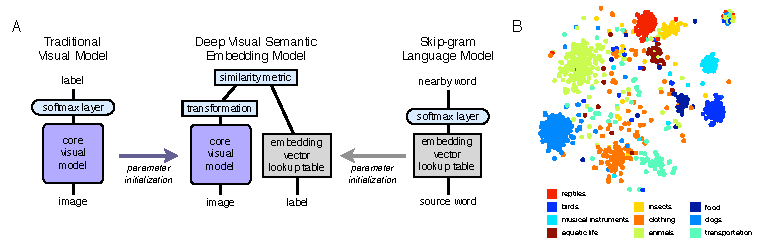
\includegraphics[width=\textwidth]{assets/devise.pdf}
  \end{center}
  \begin{itemize}
  \item Use Deep Boltzmann Machines \citep{Srivastava14}
  \item Semi-supervised learning for effective generalization from smaller data sets \citep{Kingma14b}
  \item Deep Visual-Semantic Embedding Model (DeViSE), use both unannotated text and trained image data for classification \citep{Frome13}
  \end{itemize}
\end{frame}

\begin{frame}
  \frametitle{Data}
\end{frame}

\begin{frame}
  \frametitle{Extraction of AlexNet Features}
\end{frame}

\begin{frame}
  \frametitle{Baseline LDA Results}
\end{frame}

\begin{frame}
  \frametitle{DeVISE Re-Implementation Results (Synthetic Data)}
\end{frame}

\begin{frame}
  \frametitle{Gaussian LDA Model} 
\end{frame}

\begin{frame}
  \frametitle{Gaussian LDA Results (Synthetic Data)}
  \begin{itemize}
    \item Implemented variational message passing \citep{Winn05} and stochastic variational inference using the BayesPy \citep{Luttinen14} package. 
    \item 
  \end{itemize}
\end{frame}

\begin{frame}
  \frametitle{Thank You}
  \begin{itemize}
  \item Questions?
  \end{itemize}
\end{frame}

\section{References}
\begin{frame}[t,allowframebreaks]{}
\frametitle{References}
{\small
\printbibliography
\par}
\end{frame}

\end{document}

